\documentclass[10pt,a4paper]{article}
\usepackage[utf8]{inputenc}

% \usepackage{ngerman}  % german documents
\usepackage{graphicx}  % import graphics einbinden
\usepackage{listings}  % support source code listing
\usepackage{amsmath}  % math stuff
\usepackage{amssymb} % 
\usepackage{a4wide} % wide pages
\usepackage{fancyhdr} % nice headers
\usepackage{float}
\usepackage{longtable}
\usepackage{xcolor}
\usepackage{cite}
\usepackage{fancyhdr}
\usepackage{tabularx}
\usepackage{booktabs}
\usepackage{lscape}
\usepackage{gensymb}

\usepackage[pdfpagemode=None, colorlinks=true,  % url coloring
linkcolor=blue, urlcolor=blue, citecolor=blue, plainpages=false, 
pdfpagelabels,unicode]{hyperref}

\definecolor{darkpastelgreen}{rgb}{0.01, 0.75, 0.24}
\definecolor{spirodiscoball}{rgb}{0.06, 0.75, 0.99}
\definecolor{smalt}{rgb}{0.0, 0.2, 0.6}
\definecolor{armygreen}{rgb}{0.29, 0.33, 0.13}
\definecolor{awesome}{rgb}{1.0, 0.13, 0.32}
\definecolor{bittersweet}{rgb}{1.0, 0.44, 0.37}
\definecolor{bananayellow}{rgb}{1.0, 0.88, 0.21}
\definecolor{blue}{rgb}{0.0, 0.0, 1.0}
\definecolor{red}{rgb}{1.0, 0.0, 0.0}
\definecolor{green}{rgb}{0.0, 1.0, 0.0}





\title{\Huge Bioinformatics Practicals In Sillico \\ \textbf{\normalsize BC-7107}}

%\raggedright
%
\includegraphics[width = 40mm]{img/unibe.png}\\[8ex]

\vfill
%set up names, matricle number, and email
\author{
	\noindent
	\begin{tabular}[t]{@{}l}
		\href{mailto:thibault.schowing@unifr.ch}{Thibault Schowing}\\
		\href{mailto:lio_roh@students.unibe.ch}{Lionel Rohner}\\
		\href{mailto:alain.rohrbasser.unifr.ch}{Alain Rohrbasser}\\
		\href{mailto:rares.cristea@unifr.ch}{Rares Cristea}
	\end{tabular}
		}

%\hfill
%\raisebox{\dimexpr.8\baselineskip-\height}{\includegraphics[width=32mm]{example-image}}


\begin{document}

\clearpage\maketitle
\thispagestyle{empty}
\newpage

\pagestyle{fancy}             % header
\setcounter{page}{1}

%lecture name
\newcommand{\lecture}{
	Bioinformatics Practicals In Sillico
}           

%assignment iteration
\newcommand{\assignment}{
	BC-7107
}


\setlength \headheight{25pt}
\fancyhead[R]{\begin{tabular}{r}\lecture \\ \assignment \end{tabular}}
\fancyhead[L]{HS-2019}

\part*{Introduction}



%File types used
%\begin{itemize}
%	\item \textbf{FA} The files with the .fa extension store FASTA format sequences. In this project the .fa file contains the reference genome.  
%	\item \textbf{GTF} The Gene transfer format (GTF) is a file format used to hold information about gene structure. It is a tab-delimited text format based on the general feature format (GFF), but contains some additional conventions specific to gene information. A significant feature of the GTF that can be validated: given a sequence and a GTF file, one can check that the format is correct. This significantly reduces problems with the interchange of data between groups.
%	\item \textbf{VCF} The Variant Call Format stores the gene sequence variation. By using the variant call format only the variations need to be stored along with a reference genome which make the file less redundant.
%	\item \textbf{BAM} Binary Alignment Map (BAM) is the comprehensive raw data of genome sequencing; it consists of the lossless, compressed binary representation of the Sequence Alignment Map. BAM is the compressed binary representation of SAM (Sequence Alignment Map). BAM is in compressed BGZF format.
%\end{itemize}
Bioinformatics is the application of computational technology to handle the rapidly growing repository of information related to molecular biology. Bioinformatics combines different fields of study, including computer sciences, molecular biology, biotechnology, statistics and engineering. It is particularly useful for managing and analysing large sets of data, such as those generated by the fields of genomics and proteomics.\\

In this report we focus on the bioinformatics tools for mutant analysis through three different projects; mutations in gai and spy in Arabidopsis Thaliana, mutations in Saccharomyces cerevisiae and mutations as well as Denovo assembly in Lactobacillus Helveticus. We want to sort out new mutation with these tools and learn how to design a bioinformatics test. It includes the quality test, the annotation of our sequenced genomes and various analysis of these results. Thus, everything upstream of the analysis must be properly done, using several software described thereafter. Our machines are too week in order to analyse the data and performed the bioinformatics steps, thus, we will use a cluster dedicated for this lecture, in Bern Switzerland. 




\newpage
\part*{Yeast Genome Analysis}

\section*{Introduction}

%\paragraph{Biological introduction}The budding Yeast Saccharomyces cerevisiae is a common organism used for genetics manipulation. This organism is well conserved among the eukaryote and can be used correlate with human pathways. With a genome with 16 chromosomes (haploid, Mat a or $ \alpha $) or 32 chromosomes (diploid). 99\% of the genome is without introns, make this organism handy to manipulate. 12 million bases pair and contains between 5 800 to 6 572 genes %TODO ref. 

%The homology with human is estimate to 23\%, which is a good candidate for preliminary studies regarding human pathways. The short mating time and growth is also short. Thus, the identification of potential mutant is grandly enhanced. This is a single eukaryotic organism with a division cycle of 90 minutes. Through the process of budding in which smaller daughter cells pinch, or bud, off the mother cell. Due to the microscopic size ($~$5 microM, between bacteria and human cell size) and simple growth environment, yeasts are inexpensive and easy to grow in silico. Saccharomyces cerevisiae is also no-pathogen, and forms colonies on agar plates in the laboratory in a few days with no special incubators required (best grow at 30 $ \deg $). 

The budding yeast Saccharomyces cerevisiae (S.cerevisiae) is a single-celled lower eukaryote belonging to the kingdom of fungi. Ever since its discovery, S.cerevisae has nourished human advancements in the field of fermented food products, alcoholic beverages (e.g. beer, which is the epony of S.cerevisae) and the production of biofuel.1 In addition to the contribution industrial fermentation, S.cerevisiae has become one of the most popular model organism for eukaryotic biology, due to its simple cellular architecture, cheap maintenance cost, fast growth, non-pathogenic nature (discussed in \cite{perez-torrado_opportunistic_2016}) , and homologies to human cells (e.g. ribosomes), which cannot be studied in prokaryotic model organism, such as E.coli \cite{botstein_yeast_2011}. In particular, the genetic analysis of S.cerevisiae has gained popularity in the scientific community since it was the first eukaryotic organism whose genome was fully sequenced. The haploid genome of S.cerevisiae consists of 16 linear chromosomes containing 6604 genes encoded within approximately 12 megabase-pairs (Mbp)\cite{belda_saccharomyces_2019}. The fact that genome of S.cerevisiae is quite small and almost completely void of intronic DNA, thus making it an ideal microorganism for the identification of mutations and single nucleotide polymorphisms.\\

Mating of two haploid yeast of opposite mating type (i.e. Mat a or $\alpha $) gives rise to diploid cells that possess 32 chromosomes. This is a single eukaryotic organism with a division cycle of 90 minutes. Through the process of budding in which smaller daughter cells pinch, or bud, off the mother cell. S.cerevisiae forms colonies on agar plates in the laboratory in a few days with no special incubators required (best grows at 30\degree C).\\


%todo tom 1
\textbf{TODO Thibault INTRO SERIEUSE SUR TOM1 - intro gene rapport yeast}

\paragraph{Target of Myb protein1 (Tom1)}, is a gene involved in the ribosomal biogenesis in yeast and human respectively. In human, this gene is involved in several pathways including endocytosis, endosomal transport, intracellular protein transport, neutrophil degranulation and protein transport. 
%1 
\cite{seroussi_tom1genes_1999}
%2 
\cite{seet_endofin_2004}
It is located on the ch.22 (component UP000005640) and ch.4 in human and yeast respectively. As it is well conserved among the eukaryote, we can study the gene with yeast foe the raisons explained above. In yeast specifically, TOM1 was first described as gene involved in temperature sensitivity and could be supress by STM1. 
%3 
\cite{utsugi_high_1995}
TOM1 is a hect-domain, wherein has been identified as a conserved feature of E3 ubiquitin ligases group. It regulates transcriptional activation Through effectors ADA on coactivator proteins on the DNA. The action of TOM1 is to regulate through ubiquitination the temperature sensitivity. 
%4 
\cite{saleh_tom1p_1998}
A tom1-1 mutant has been isolated, and under electron microscopy and indirect immunofluorescence microscopy, it has been shown that the large nucleus contains duplicated DNA and short spindle and structures fragmentations.5. This show that the disruption of the system that impact the nuclear transport and the cell division in the G1 phase. 
%2 
\cite{seet_endofin_2004}
%5 
\cite{utsugi_yeast_1999}
TOM1 encode for a large 380KDa proteins with a hect-domain at its C terminus (homologous to E6-AO C terminus). Site-directed mutagenesis of the conserved cysteine residue (tom1C3235A) in the hect-domain, supposed to be necessary for thioester-bond formation with ubiquitin, abolished the gene function. After a test with the over production of a myc-tagged ubiquitinRA, it shows that TOM1 is a ubiquitin ligase.
%5 
\cite{utsugi_yeast_1999}
More recently, TOM1 has been described as a fundamental macromolecular machine. The ribosomes biogenesis is much more complex in eukaryote cells as in bacteria, and it is involved in several fundamental cellular processes, including growth and cell division.
%7 
\cite{dinman_eukaryotic_2009}
Ribosomes are subunits assemblage allowing the production of proteins. Subunits are made of RNA (rRNA) and specifies proteins (r-proteins) (Saccharomyces cerevisiae: 40S [18S rRNA, 33 RPs]; 60S [25S, 5.8S, 5S rRNA, 46 RPs]–Escherichia coli: 30S [16S rRNA, 21 RPs]; 50S [23S, 5S rRNA, 34 RPs]).
%10 
\cite{kressler_driving_2010}
Recent studies have shown that defect in the biogenesis linked to a wide range of hereditary diseases like Alzheimer’s and anemia.
%9 citer rapport ??????
%11 
\cite{makioka_immunolocalization_2016}
Ribosomes are a mixture of almost 80 different protein and stick together through a scaffold made by the RNA as explain above. Each protein is express in one copy and each of these proteins are needed to assemble the ribosomes. However, the number of steps needed for the biogenesis is large and not totally known. Moreover, it is impossible for a cell to produce the exact number of the needed proteins, furthermore the same number of copies of all the proteins in a ribosome
%8 
\cite{sung_conserved_2016}
It will build up the number needed and then degrade the leftover, wherein are ubiquinined by TOM1 and degraded in lysosomes. We can say that TOM1 act as a quality control on this mechanism during the anabolism and division phases of the cells, leading to a week and crucial homeostasis
%8 
\cite{sung_conserved_2016}
Ribosome biogenesis is an intricate process involving many chaperons and assembly factors ($>$200 factors) and snoRNAs (75)
%10 
\cite{kressler_driving_2010}
Two subunits are part of the final ribosomes, the 40S has one rRNA (18S) and 33 r-proteins. The 60S (comprises three rRNAs (25S, 5.8S, 5S) and 47 r-proteins subunit 
%9 citer rapport ?????
%10 
\cite{kressler_driving_2010}\\

\textbf{todo ci-dessous ça veut rien dire, la 2ème phrase est pas finie}\\

The assembly and maturation of the ribosomes passes from the nucleus to the cytosol. ATP-dependent RNA helicases and three AAA-type ATPases (ATPases associated with various cellular activities). This suggests that the energy derived by these enzymes is required for ribosomes assembly. The absence of one of these proteins might stall ribosome biogenesis and terminate cell growth even under optimal growth conditions 
%7 
\cite{dinman_eukaryotic_2009}
%10 
\cite{kressler_driving_2010}.\\

To summarize, TOM1 is necessary to the ribosome’s biogenesis and the elimination of the leftover building blocks by ubiquitination. Thus, the aim of this project is to identify the suppressor of this gene by high sequencing throughput with bioinformatics tools. \\

\textbf{TODO on en fait référence nule part à cette figure -> nécessaire ?}
\begin{figure}[h]
	\centering
	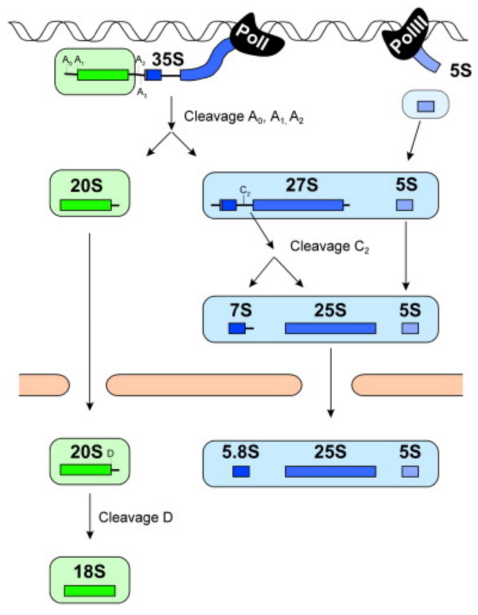
\includegraphics[width=0.4\linewidth]{img/tom1Intro}
	\caption{Simplified overview of the major steps in pre-rRNA processing.}
	\label{fig:tom1intro}
\end{figure}


%\paragraph{\textit{tom1}} The deletion of Tom1 has been associated with aggregation of ribosomal proteins, which results in a temperature-sensitive phenotype of S.cerevisiae that renders them incapable of growing at temperature exceeding 20\degree C. \\

%The aim of this study is to screen several $ \Delta $tom1 \textit{S.cerevisiae} strains for mutations in genes associated to tom1 (positive and negative regulators) and genes coding for riboproteins. \\

%In this project, we present a number of potential candidates that might help deciphering the temperature-sensitive phenotype of $ \Delta $tom1 \textit{S.cerevisiae}.


\section*{Methods}

\paragraph{Quality control of sequences} The high throughput sequencing method isn’t infaillble, so the data will have contaminants, badly read sequences due to the intensity of the fluorescent signal, or the quality of the reagents that have a decaying quality with the number of sequencing cycles over time\cite{abnizova_computational_2017}. These errors might add a lot of false signals, useless extrawork, and complicate the data analysis, therefore we need to get rid of them. 
In order to check for the quality of the data, we use the tool : \textit{fastqc}\cite{andrews2012} which will help us visualize our fasta file given by the sequencer. \\


\paragraph{Trimming and bad quality removal } After the quality control check, we used the tool \textit{trimmomatic}\cite{bolger_trimmomatic:_2014} with the given parameters of MINLEN : 130 to trim down the bad quality ends of the reads, keeping at least 130bp of the trimmed read, and the parameter SLIDINGWINDOW:4:15, thus removing the reads that have an average base pair quality score lower than 15. The next step was checking if the quality of the data has improved after the trimming process, by using again fastqc, on the trimmomatic fastq file output.

\paragraph{Sequence alignment against reference} Since the fasta files gives no information about the sequences position in the yeast genome, we had to align all of the reads against the fasta file of a known yeast genome, or most likely a consensus of a yeast genome, containing the positional information.\\
 
However, in order to do that, we first had to index the reference fasta using the \textit{bwa index} tool\cite{li_fast_2010}, which is a way of giving a sort of table of contents of our reference fasta file (in our case the \href{https://www.ensembl.org/Saccharomyces_cerevisiae/Info/Index}{R64-1-1.92.fa}), that is used by the burrows-wheeler aligner algorithm. Subsequently, we used the \textit{bwa mem} tool in order to align our sequenced data against the reference. Then, we have converted all the SAM\cite{li_sequence_2009} files containing our aligned sequences, into BAM files, a compressed binary format easier to work with.
 
\paragraph{Variant calling and annotation}
This has been done using only \textit{samtools mpileup}, that took our reference file, and the aligned BAM files as an input, and gave us the binary format of the \textit{Variant Calling Format} files (.vcf). Then we used \textit{bcftools} to convert them into vcf.gz files. This method was prefered considering the fact that our genome is a haploid yeast genome, and it doesn’t need a complicated algorithm as used by the \textit{GATK} pipeline. The \textit{tabix}\cite{li_tabix:_2011} tool was used on the vcf files, in order to index them properly.\\

In order to annotate the variants given by the vcf files, we had to use \textit{SNPeff} tool on the vcf files that were merged together with all their indexes, and we also kept only the variants that were found in less than all 4 strains that we had to analyse, since we had to filter through all the variants that were different from the reference. The variants interesting to us, are indeed the ones that are specific to one of the mutants, and that’s why we had to filter this way.\\

The results were then visualized by either reading the vcf files in xcel or in IGV.\\


%todo 
\textbf{TODO Lionel WIP Gene TOM ou autre polymorphisme trouvé à décrire dans le fichier vcf.}











\newpage
\part*{Arabidopsis Thaliana Genome Analysis}

\textbf{TODO ALAIN: REVOIR INTRO, MERGE SPY}\\

\textbf{TODO LIONEL: CHANGER IMAGE}

\section*{Introduction}
The plant Arabidopsis thaliana is a genetic model worldwide used in plant biology since 1995, when it has been promoted as model for molecular genetics. The genome is entirely sequenced in 200. ATH is a diploid organism of 114,5 to 125 million base pairs within 5 chromosomes (haploid). The germination to mature seed is done about 6 weeks and easy to cultivate in restricted space and produce a lot of seed. A wide range of mutants are already available and it growth from year to another through multinational research community of academic, government and industry laboratories. The importance of ATH is crucial and invaluable resources to fight the loss of crops due to plants diseases.


%
%
%


\paragraph{GAI} 

Gibberellic-Acid Insensitive (GAI) is a gene in Arabidopsis thaliana in chromosome 1 which is involved in the regulation of plant growth.  Precisely, it mediated the input signals and module the growth by decreasing the responsiveness to gibberellin\cite{peng_arabidopsis_1997}.
%http://genesdev.cshlp.org/content/11/23/3194.short
Gibberellin is a tetracyclic diterpenoid growth factor and influence essentially the stem elongation and other plant developmental processes\cite{hooley_gibberellins:_nodate}.
%https://link.springer.com/article/10.1007%2FBF00016489
The main mutation involved a deletion of a 17 amino acid segment. The gai allele contains a deletion of 51-bp from within the GAI ORF ,from close to the N terminus and confers a dominant dwarf phenotype. The mutation take place at the DNA-binding transcription factor activity and causes a dwarf phenotype. It acts as a repressor and a coactivator of the zinc finger transcription factors GAF1/IDD2 and ENY/IDD1 in regulation of gibberellin homeostasis and signalling of the gibberellin (GA) signalling pathway. The GAI (gai1-1 and gai 1-2, two mutations on the same gene) protein as normally a length of 533 AA and is normally located in the nucleus. The deleted segment is shown in yellow for DELLA, the common one\cite{peng_arabidopsis_1997}\cite{lee_gibberellin_2002}.
%doi:10.1101/gad.11.23.3194
%http://genesdev.cshlp.org/content/16/5/646
If it is mutated (gai) and the plant growth better, it is a gain of function gene, in contrary it is a loss of function. The cellular gai’s component is in the nucleus and is described as a transcription region of DNA and bind it directly. The mutation in SPY (spy) is a suppressor of gai, conferring to the plant a normal phenotype. GA-deficient Arabidopsis mutants display characteristic phenotypes, including dark green leaves and a dwarf growth habit attributable to reduced stem elongation\cite{peng_arabidopsis_1997}.
%http://genesdev.cshlp.org/content/11/23/3194.short
The gai mutation affects GA reception or subsequent signal transduction and does not result in GA deficiency\cite{hooley_gibberellins:_nodate}.
%https://link.springer.com/article/10.1007%2FBF00016489


\begin{figure}[H]
	\centering
	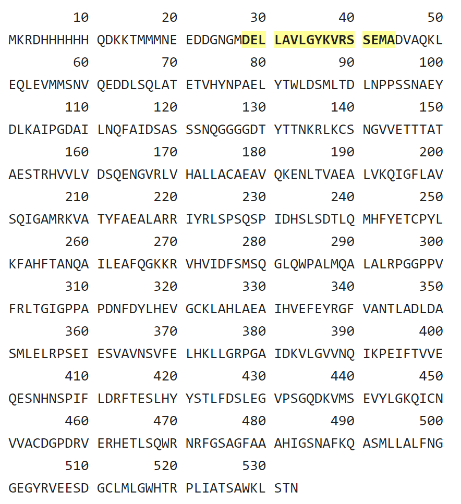
\includegraphics[width=0.4\linewidth]{img/dellamutation}
	\caption{The DELLA protein GAI comes from the GRAS family protein 3 and located on the chromosome 1, locus:2006747 AT1G14920. Call DELLA because of the 17 AA deleted.}
	\label{fig:dellamutation}
\end{figure}





\paragraph{SPY}
For spy, three independent recessive mutations at the SPINDLY (SPY) locus of Arabidopsis confer resistance to the gibberellin (GA) biosynthesis inhibitor paclobutrazol. Paclobutrazol or $ \alpha $-tert-Butyl-$ \beta $-(4-chlorobenzyl)-1H-1,2,4-triazole-1-ethanol, is a plant growth retardant. It is an antagonist of the plant hormone gibberellin. It works by inhibiting gibberellin biosynthesis by inhibiting endoplasmic reticulum monooxygenases. Relative to wild type, spy mutants exhibit longer hypocotyls, leaves that are a lighter green colour, increased stem elongation, early flowering, parthenocarpy, and partial male sterility. All of these phenotypes are also observed when wild-type Arabidopsis plants are repeatedly treated with gibberellin A3 (GA3). The spy-1 allele is partially epistatic to the ga1-2 mutation, which causes GA deficiency. In addition, the spy-1 mutation can simultaneously suppress the effects of the ga1-2 mutation and paclobutrazol treatment, which inhibit different steps in the GA biosynthesis pathway. This observation suggests that spy-1 activates a basal level of GA signal transduction that is independent of GA\cite{lee_gibberellin_2002}.
%http://genesdev.cshlp.org/content/16/5/646


%TODO remplacer par figure à Lionel
% \label{fig:gaspypathway}

\begin{figure}[H]
	\centering
	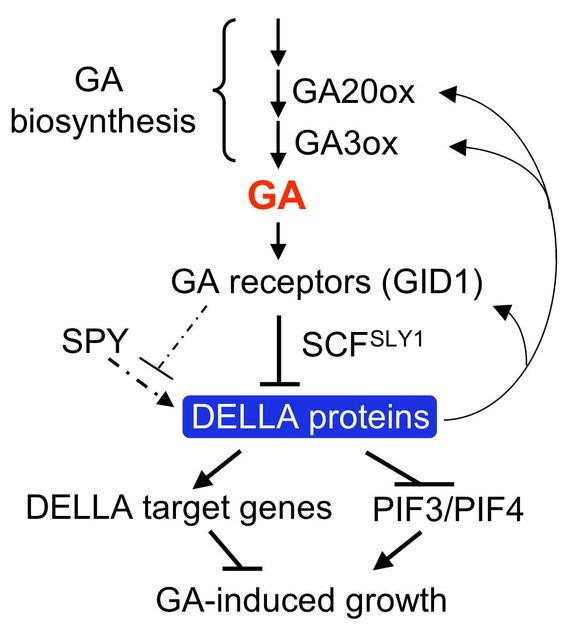
\includegraphics[width=0.4\linewidth]{img/GASPYpathway}
	\caption[GAI and SPY pathways]{https://www.ncbi.nlm.nih.gov/pmc/articles/PMC3243332/figure/i1543-8120-64-1-1-f21/}
	\label{fig:gaspypathway}
\end{figure}


\section*{Methods} \textbf{TODO Rares}

\section*{Results} \textbf{TODO Rares}

\paragraph{Discussion}


%%%%%%%%%%%%%%%%%%%%%%%%%%%%%%%%%%%%%%%%%%%%%%%%%%%%%%%%%
\newpage
\part*{Lactobacillus Heleveticus Genome Assembly}
\section*{Introduction}

%TODO table abreviation (LAB)(PGHs)



The diverse bacteria involved in cheese production are essential for the texture and taste development but also, during the ripening process, the microbial changes helps to kill pathogens and reduce spoilage micro-organisms. \textit{Lactobacillus helveticus} is a thermophilic lactic acid bacterium (LAB) used in the dairy industry as a starter or an adjunct culture for cheese manufacture\cite{jebava_nine_2011}. By releasing \textbf{peptidoglycan hydrolases}(PGHs), it has the ability to digest the bacterial cell wall (gram+) inducing death of surrounding bacteria but also its autolysis. \\

The genomic plasticity of \textit{Lactobacillus helveticus} leads to a high variation in PGHs activity from one strain to another. In a previous study, the activity of a PGH with an estimated size of 30kDa was tested by zymography in nine strains of \textit{Lactobacillus helveticus} of which six were sequenced (see figure \ref{fig:zymography}). Two phenotypes were shown: phenotype A exhibits PGH activity (strains \textbf{FAM8102c1c1}, \textbf{FAM23285} and \textbf{FAM19191}) and phenotype B does not (strains \textbf{FAM22016}, \textbf{FAM1450} and \textbf{FAM1213}).\\

The aim of this work was to detect potential genomic differences involved in the two different phenotypes by sequencing, assembling and compare the genome of the six strains using a previously annotated reference genome of \textit{Lactobacillus helveticus} (\href{https://www.ncbi.nlm.nih.gov/genome/?term=NC_010080}{NC\_010080}). A potential candidate present only in the strains expressing a PGHs activity suggests that it might have been acquired by a viral insertion. 

  
%TODOOOOOOOOOOOOOOO

% BLASTP the protein sequence to see it comes from a phage !

\section*{Methods}

%TODO cite SOAPdenovo, Spades and Abyss
\paragraph{Sequencing and genome assembly}
The six \textit{Lactobacillus helveticus} strains \textbf{FAM8102c1c1}, \textbf{FAM23285}, \textbf{FAM19191}, \textbf{FAM22076}, \textbf{FAM1450}, \textbf{FAM1213}  were sequenced by Illumina sequencing. The following tasks were performed using the cluster provided by the University of Bern.  \textit{FastQC}\cite{andrews2012} was used to check the quality of the reads and \textit{Trimmomatic}\cite{bolger_trimmomatic:_2014} to filter out bad quality reads. \textit{SOAPdenovo} as well as \textit{Spades} were used to perform the genome assembly with the reads of each strains. For \textit{SOAPdenovo} the k-mer sizes were set to 95, 85, 75 and 65. For \textit{Spades} k-mere sizes were set to 21, 33, 55, 77 and 99 (default values). The four assemblies of SOAPdenovo and the assembly of Spades were compared using Abyss with a maximum number of contigs set to 1000. The best genome assemblies with the bigger N50 and a approximate genome size of 20Mbp (Genome size of \textit{Lactobacillus helveticus}) were then chosen\footnote{Due to the temporary unavailability of the cluster, this operation has been performed by L. Falquet and the results were provided to the students afterwards.}.


\paragraph{Genome annotation and pan-genome analysis}
We used the \textit{PROKKA} pipeline\cite{seemann_prokka:_2014} to annotate the genome of the six best assemblies and the reference genome for \textit{Lactobacillus helveticus} \href{https://www.ncbi.nlm.nih.gov/genome/?term=NC_010080}{NC\_010080}. \textit{PROKKA} is an automated pipeline that annotates prokaryotic genomes. It locates open reading frames ans RNA regions on contigs and translates it to protein sequences, searching for protein homologues in public databases. The resulting standards \href{https://www.ensembl.org/info/website/upload/gff.html}{.gff} files containing the annotated genome for each strain are then used by \textit{Roary}\cite{page_roary:_2015} to generate a pan-genome of the six strains. The result was then visualized with \textit{Phandango}\cite{hadfield_phandango:_2018} allowing visualisation of phylogenetic tree, associated metadata and genomic information.


\paragraph{Extraction of the genes for each phenotypes} Grep was applied to the files generated by \textit{Roary} to extract the nine PHG's \cite{jebava_nine_2011} labelled "Lhv\_" with \textit{PROKKA} (table \ref{tab:resultCommonLhv}). The set of genes found in strains expressing phenotype A was then compared to the set of gene showing phenotype B. In table \ref{tab:resultPGHexpr} we have the two PGHs present only in the three strains expressing the PGHs activity. The nucleotide sequences were then converted to amino acid sequences for further comparison. 
%TODOAAAAAAAAAAAAAAAAAAAAa


\begin{figure}
	\centering
	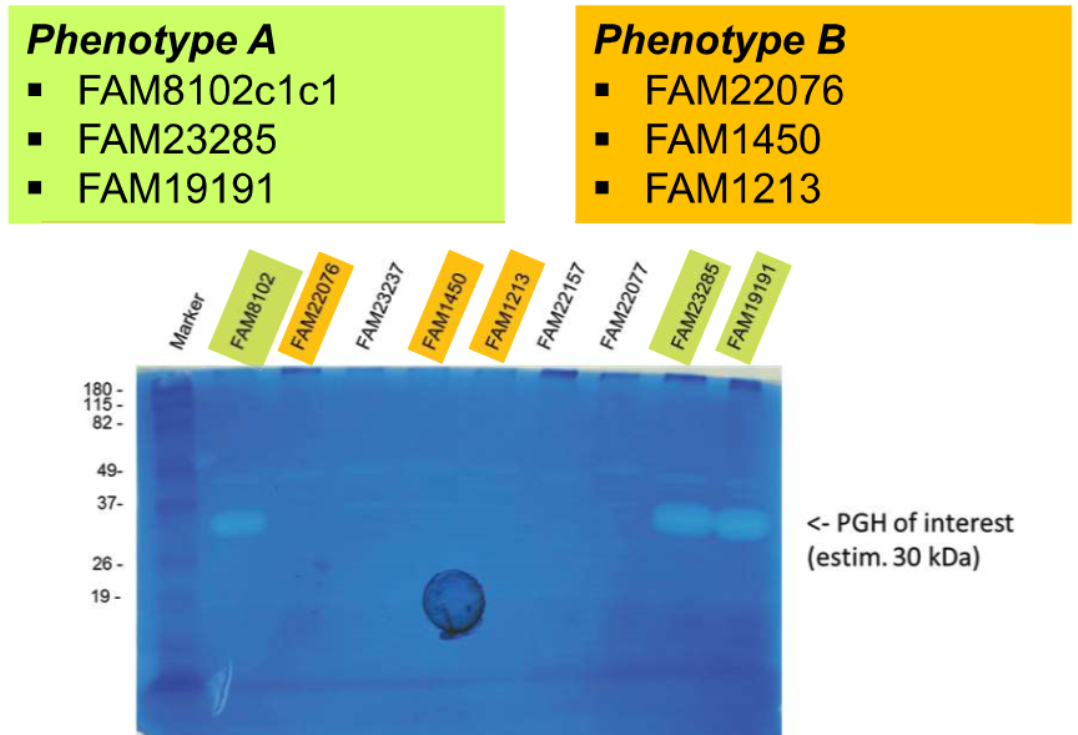
\includegraphics[width=0.6\linewidth]{img/zymography}
	\caption[The two phenotypes expressed by the six strains]{Phenotype A is expressing an active peptidoglycan hydrolase and phenotype B is not.}
	\label{fig:zymography}
\end{figure}


\newpage
\section*{Results}



%TODO fix images


\begin{table}[htbp]
	\centering
	\begin{tabularx}{\linewidth}{|X|X|X|X|X|X|}
		\hline
		\textbf{Gene} & \textbf{Annotation} & \textbf{Avg group size nuc} & \textbf{FAM19191\_ 1K} & \textbf{FAM23285\_ 1K} & \textbf{FAM8102\_ 1K}\\
		 \hline
		%group\_1899 & Lhv\_2053 Lysin (L.crispatus) pseudogene in L.helveticus & 830/ 30 kDa & FAM19191\_ 1K\_00615 & FAM23285\_ 1K\_00607 & FAM8102\_ 1K\_00746 \\
		%\hline
		group\_2348 & Lhv\_2053 Lysin (L.crispatus) pseudogene in L.helveticus & 1121/ 41 kDa & FAM19191\_ 1K\_00069 & FAM23285\_ 1K\_00060 & FAM8102\_ 1K\_00069 \\
		\hline
		group\_2372 & Lhv\_2053 Lysin (L.crispatus) pseudogene in L.helveticus & 893/ 33 kDa & FAM19191\_ 1K\_00397 & FAM23285\_ 1K\_00499 & FAM8102\_ 1K\_00565 \\
		\hline	
	\end{tabularx}
	\caption{Genes present only in the three strains with a PGH activity.}
	\label{tab:resultPGHexpr}
\end{table}

According to figure \ref{fig:zymography}, the PGH involved is approximately 30kDa thus matches with group 2372. Looking at the alignment of the amino acid sequences (Figure \ref{fig:alignmentgrp2372}) we see that the sequences are identical thus showing a great conservation between the three strains. \\




\begin{figure}
	\centering
	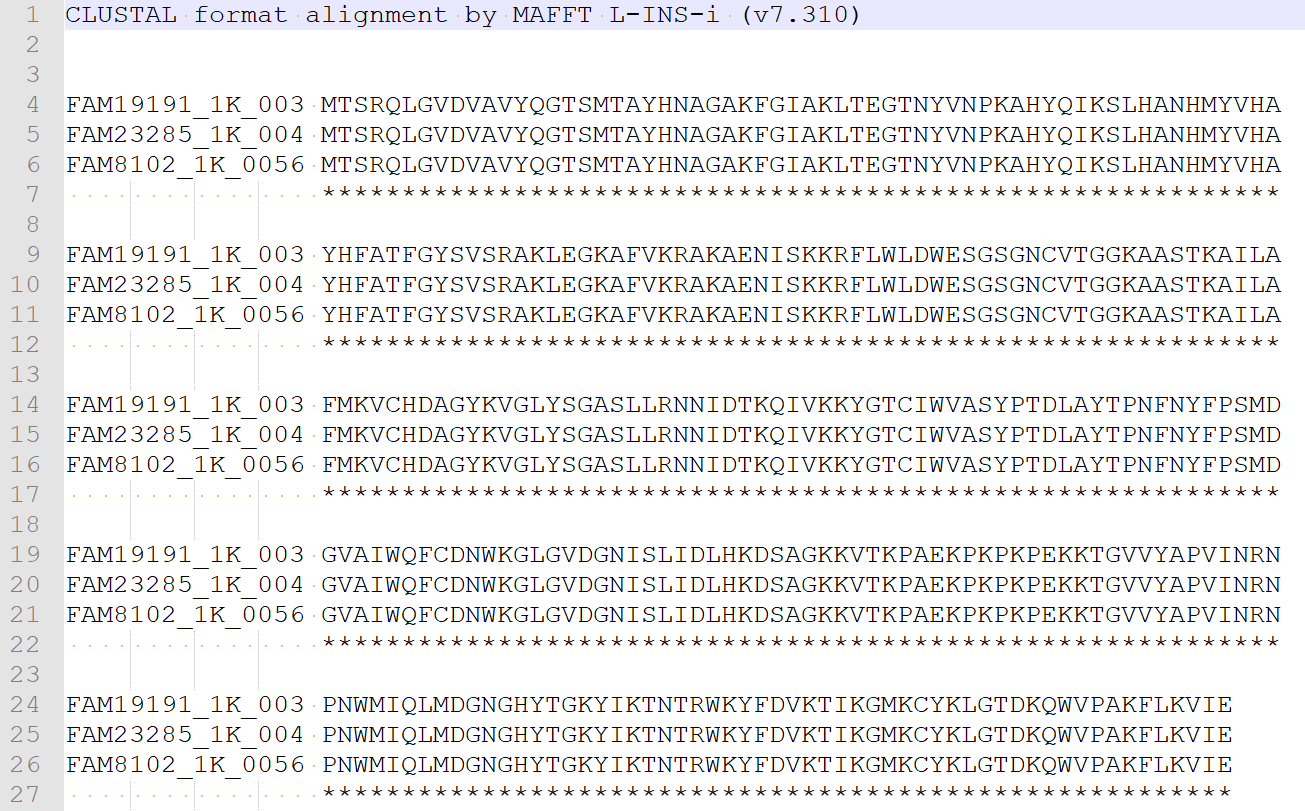
\includegraphics[width=0.6\linewidth]{img/AlignmentGrp2372}
	\caption{Alignment of amino acid sequences of group 2372 for the three strains.}
	\label{fig:alignmentgrp2372}
\end{figure}



%TODO align with mauve to reference (see script)

%TODO check this paper : https://www.ncbi.nlm.nih.gov/pmc/articles/PMC6606699/ 




%todo discuss the results
\paragraph{Discussion} We can see that PGHs are present in all strains (table \ref{tab:resultCommonLhv}), therefore the phenotype observed in the figure \ref{fig:zymography} is not due to an absence of PGH.\\

Using BLASTp\cite{altschul_gapped_1997} with default parameters, the protein was searched to be a particular lysin (\href{https://www.ncbi.nlm.nih.gov/protein/1325986555}{WP\_101853908.1}) encoded by the pneumococcal bacteriophage Cp-1\cite{martin_pneumococcal_1998}. To look further into this sequence, we could use PHASTER \cite{arndt_phaster:_2016}, the PHAge Search Tool - Enhanced Release, which helps identifying and annotate prophage sequences within bacterial genomes and plasmids. 

%todo Phaster analysis

% Reverse translation: https://www.bioinformatics.org/sms2/rev_trans.html
% Phaster analysis bookmarked 
%todo finish faster

\newpage
\bibliography{mybib}{}
\bibliographystyle{ieeetr}

\appendix
\section{Supplementary figures Yeast Genome Analysis}


\section{Supplementary figures Arabidopsis Thaliana Genome Analysis}


\section{Supplementary figures Lactobacillus Helveticus Genome Assembly}

\begin{landscape}
	\begin{table}[]
		\begin{tabularx}{\linewidth}{|l|l|X|X|X|X|X|X|}\hline
			Gene & Annotation & FAM1213 1K & FAM1450 1K & FAM19191 1K & FAM22076 1K & FAM23285 1K & FAM8102 1K \\\hline
			
			group\_1103 & \begin{tabular}[c]{@{}l@{}}Lhv\_0549 \\N-acetylmuramidase \end{tabular} & FAM1213\_ 1K\_01187 & FAM1450\_ 1K\_00785 & FAM19191\_ 1K\_01147 & FAM22076\_ 1K\_00934 & FAM23285\_ 1K\_01072 & FAM8102\_ 1K\_01185 \\\hline
			
			group\_1218 & \begin{tabular}[c]{@{}l@{}}Lhv\_1433 Lysin \end{tabular} & FAM1213\_ 1K\_01833 & FAM1450\_ 1K\_00044 & FAM19191\_ 1K\_01884 & FAM22076\_ 1K\_01582 & FAM23285\_ 1K\_01903 & FAM8102\_ 1K\_01986 \\\hline
			
			group\_3457 & \begin{tabular}[c]{@{}l@{}}Lhv\_0649 Lysozyme \end{tabular} & FAM1213\_ 1K\_00895 & FAM1450\_ 1K\_00838 & FAM19191\_ 1K\_01232 & FAM22076\_ 1K\_00917 & FAM23285\_ 1K\_01191 & FAM8102\_ 1K\_01268 \\\hline
			
			group\_852 & \begin{tabular}[c]{@{}l@{}}Lhv\_1295 \\Enterolysin M23 \\family peptidase \end{tabular} & FAM1213\_ 1K\_00043 & FAM1450\_ 1K\_01113 & FAM19191\_ 1K\_00150 & FAM22076\_ 1K\_00164 & FAM23285\_ 1K\_00217 & FAM8102\_ 1K\_00225 \\\hline
			
			group\_862 & \begin{tabular}[c]{@{}l@{}}Lhv\_1059 \\LysM \\peptidoglycan-binding\\ domain-containing \\protein\end{tabular} & FAM1213\_ 1K\_00147 & FAM1450\_ 1K\_00238 & FAM19191\_ 1K\_00248 & FAM22076\_ 1K\_00274 & FAM23285\_ 1K\_00308 & FAM8102\_ 1K\_00381 \\\hline
			
			group\_993 & \begin{tabular}[c]{@{}l@{}}Lhv\_1433 Lysin \end{tabular} & FAM1213\_ 1K\_00691 & FAM1450\_ 1K\_01203 & FAM19191\_ 1K\_01800 & FAM22076\_ 1K\_00088 & FAM23285\_ 1K\_01748 & FAM8102\_ 1K\_01891 \\\hline
			
			group\_995 & \begin{tabular}[c]{@{}l@{}}Lhv\_0191 \\Amidase \end{tabular} & FAM1213\_ 1K\_00700 & FAM1450\_ 1K\_00303 & FAM19191\_ 1K\_00506 & FAM22076\_ 1K\_00064 & FAM23285\_ 1K\_00566 & FAM8102\_ 1K\_00638 \\\hline
			
			group\_1862 & \begin{tabular}[c]{@{}l@{}}Lhv\_2053 Lysin \\(L.crispatus) pseudogene\\   in L.helveticus\end{tabular} &  & FAM1450\_ 1K\_00045 & FAM19191\_ 1K\_01885 & FAM22076\_ 1K\_01583 & FAM23285\_ 1K\_01904 & FAM8102\_ 1K\_01987 \\\hline
			
			group\_1899 & \begin{tabular}[c]{@{}l@{}}Lhv\_2053 Lysin \\(L.crispatus) pseudogene\\   in L.helveticus\end{tabular} &  & FAM1450\_ 1K\_00267 & FAM19191\_ 1K\_00615 & FAM22076\_ 1K\_00716 & FAM23285\_ 1K\_00607 & FAM8102\_ 1K\_00746 \\\hline
			
			group\_1344 & \begin{tabular}[c]{@{}l@{}}Lhv\_1307 \\Enterolysin M23 \\family peptidase \end{tabular} &  &  & FAM19191\_ 1K\_00162 & FAM22076\_ 1K\_00152 & FAM23285\_ 1K\_00229 & FAM8102\_ 1K\_00237 \\\hline
			
			group\_1345 & \begin{tabular}[c]{@{}l@{}}Lhv\_0190 \\N-acetylmuramidase \end{tabular} &  &  & FAM19191\_ 1K\_00507 & FAM22076\_ 1K\_00063 & FAM23285\_ 1K\_00565 & FAM8102\_ 1K\_00639 \\
			\hline
		\end{tabularx}
		\caption{PGHs in common between all strains. Extracted from the files generated by \textit{Roary} and labeled "Lhv\_" by \textit{PROKKA}.}
		\label{tab:resultCommonLhv}
	\end{table}
\end{landscape}


\end{document}